\documentclass[12pt]{article}
\author{Alex Ho}
\title{FYS4150 - Computational Physics \\ Project 3}
\usepackage{listings}
\usepackage{graphicx}
\usepackage{verbatim}
\usepackage{amsmath}
\usepackage[utf8]{inputenc}
\usepackage{xcolor}
\usepackage{hyperref}

\lstset{
language=Python,
basicstyle=\ttfamily,
otherkeywords={self},             
keywordstyle=\ttfamily\color{blue!90!black},
keywords=[2]{True,False},
%keywords=[3]{ttk},
keywordstyle={[2]\ttfamily\color{blue!90!black}},
emph={MyClass,__init__},          
emphstyle=\ttfamily\color{red!80!black},    
stringstyle=\color{blue!90!black},
showstringspaces=false,
commentstyle=\color{blue!90!black},
breaklines=true,
tabsize=3,
moredelim=**[is][\color{blue}]{@}{@}
}

\begin{document}
\maketitle
\subsection*{3a)}
\subsection*{3b)}
Implementing the Euler and Verlet method is quite easy. We have the Euler method as
\begin{align*}
x_{i+1} = x_i + v_idt \\
v_{i+1} = v_i + a_idt
\end{align*}
One needs to calculate the acceleration $a_i$ using the discretized equations that we have previously shown. One can also implement a more precise method, the Euler Cromer's method, which is given as
\begin{align*}
v_{i+1} = v_i + a_idt \\
x_{i+1} = x_i + v_{i+1}dt
\end{align*}
Which is almost the same as the Euler method, however, the position now depends on the new velocity $v_{i+1}$. Unlike the Euler method, we now need to calculate the new velocity before calculating the new position. In the Euler method, we did not have to take this into account. In the C++ program, the ordering of the position and velocity calculation are swapped for these two methods, and we will see later that this will give two different results.

The next method we will look at is the Verlet method. It is given as
\begin{align*}
x_{i+1} = x_i + v_idt + \frac{dt^2}{2}a_i\\
v_{i+1} = v_i + \frac{dt}{2}\left(a_{i+1} + a_i \right)
\end{align*}
Implementing this may be a little tricky. Calculating the position is straight forward, but the velocity now depends on $a_{i+1}$ and $a_i$. To bypass this problem, we will have to save $a_i$ so its own variable and then calculate the new acceleration $a_{i+1}$ using the new calculated position $x_{i+1}$. 

\subsection*{3c)}
The initial velocity of Earth is retrieved by data from NASA.

One can assume that the total energy for the whole system is conserved as the total energy will confined within this system. That is, we think of this system that is in a box. The energy for this system will not leave the box, thus the energy is conserved. We are also not taking into account of gravitational waves, which have some energy as well.

Another way to determine that the energy must be conserved is because the forces in this system are conservative.

We will now test the Euler and Verlet method, presented earlier, to solve the Earth-Sun system. Figure 1 shows the plots of the Earth-Sun system using Euler (top image) and Verlet method (bottom image). As we can see, the Verlet method gives a more precise and stable Earth orbit, whereas the Euler method gives a less stable Earth orbit.

For the C++ program, the time difference between these two methods are almost negligible for a small number of time steps. The Verlet method had to run roughly 2 times longer compared to the Euler method, which is not surprising due to the increased number of FLOPS required to solve one time step. However, as we saw from the plots, the extra time it took for the Verlet method gave a much better result than the one using Euler method.

\begin{lstlisting}
@Running Euler method
Time elapsed for Euler method:0.1s
Data saved to: Earth_Sun_sys_euler.txt

Running Euler Cromer method
Time elapsed for Euler Cromer method:0.097s
Data saved to: Earth_Sun_sys_eulercromer.txt

Running Verlet method
Time elapsed for Verlet method:0.202s
Data saved to: Earth_Sun_sys_verlet.txt@
\end{lstlisting}

One can also use the Euler Cromer method to solve these systems. A plot of the Earth-Sun system using the Euler Cromer method can be found in the appendix. As we can see, the results practically identical to the Verlet method. The time it took to finish the Euler Cromer method was just a tiny bit faster than the ordinary Euler method.
\begin{figure}[hbtp]
\centering
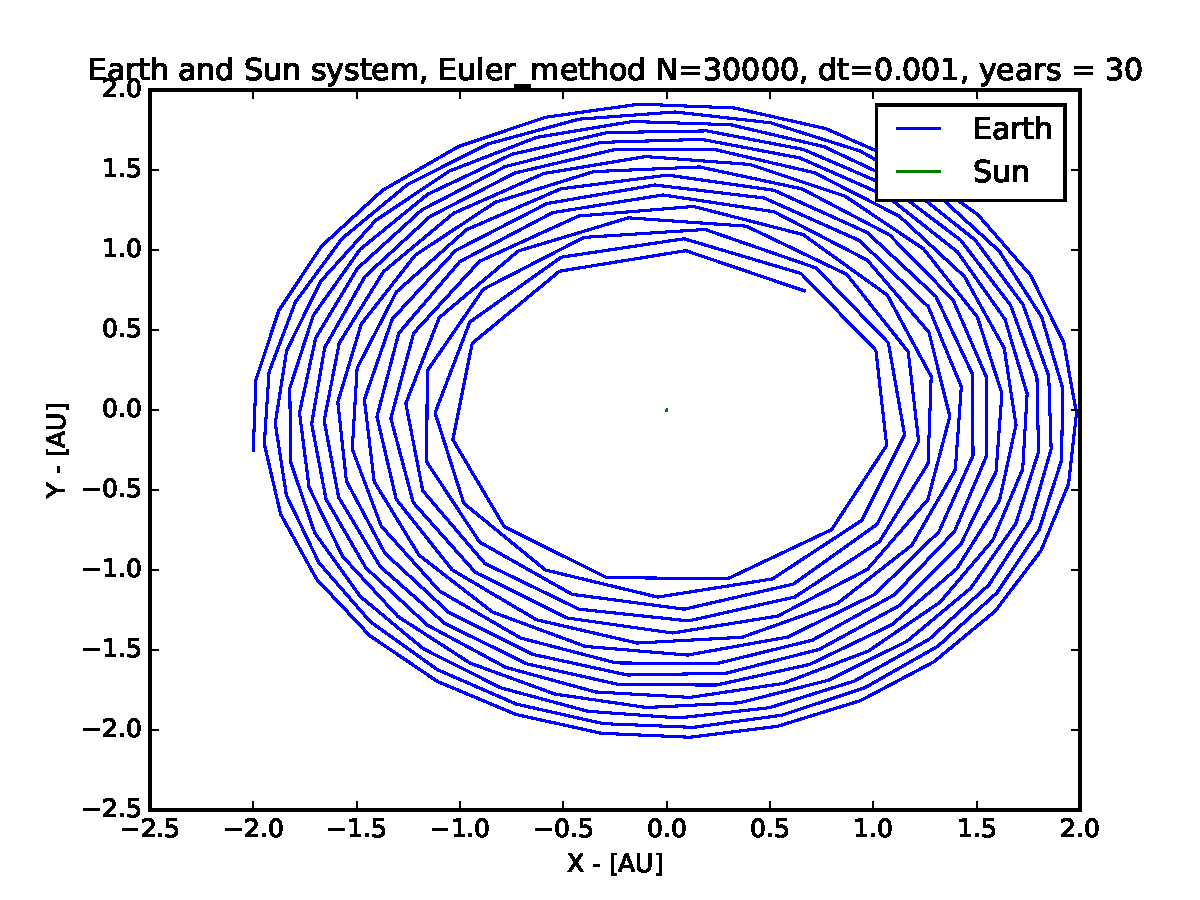
\includegraphics[width=\linewidth]{Plots/Earth_Sun_Euler_method.pdf}
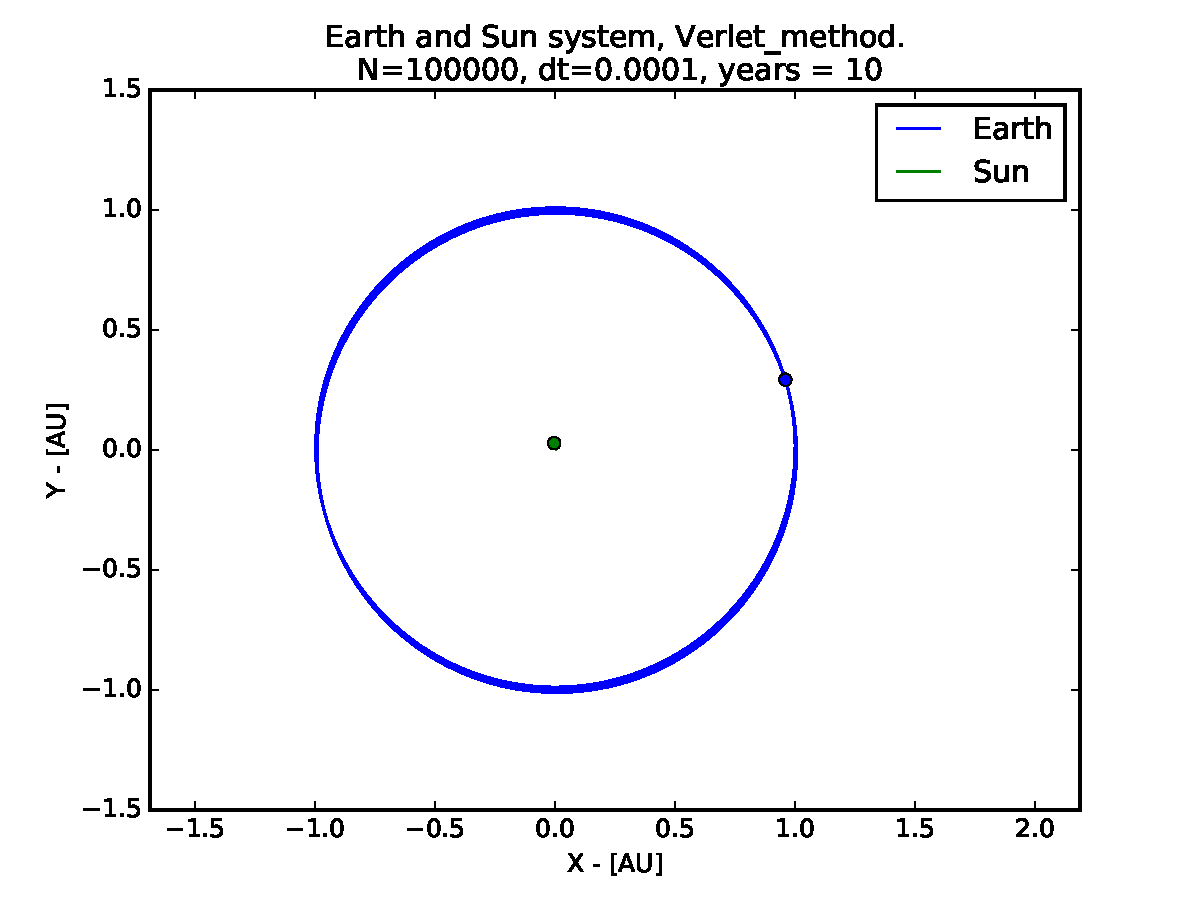
\includegraphics[width=\linewidth]{Plots/Earth_Sun_Verlet_method.pdf}
\caption{Comparison of Euler and Verlet method for the Earth-Sun system}
\end{figure}

\subsection*{3d)}
\subsection*{3e)}

\section*{Appendix}
\begin{figure}[hbtp]
\centering
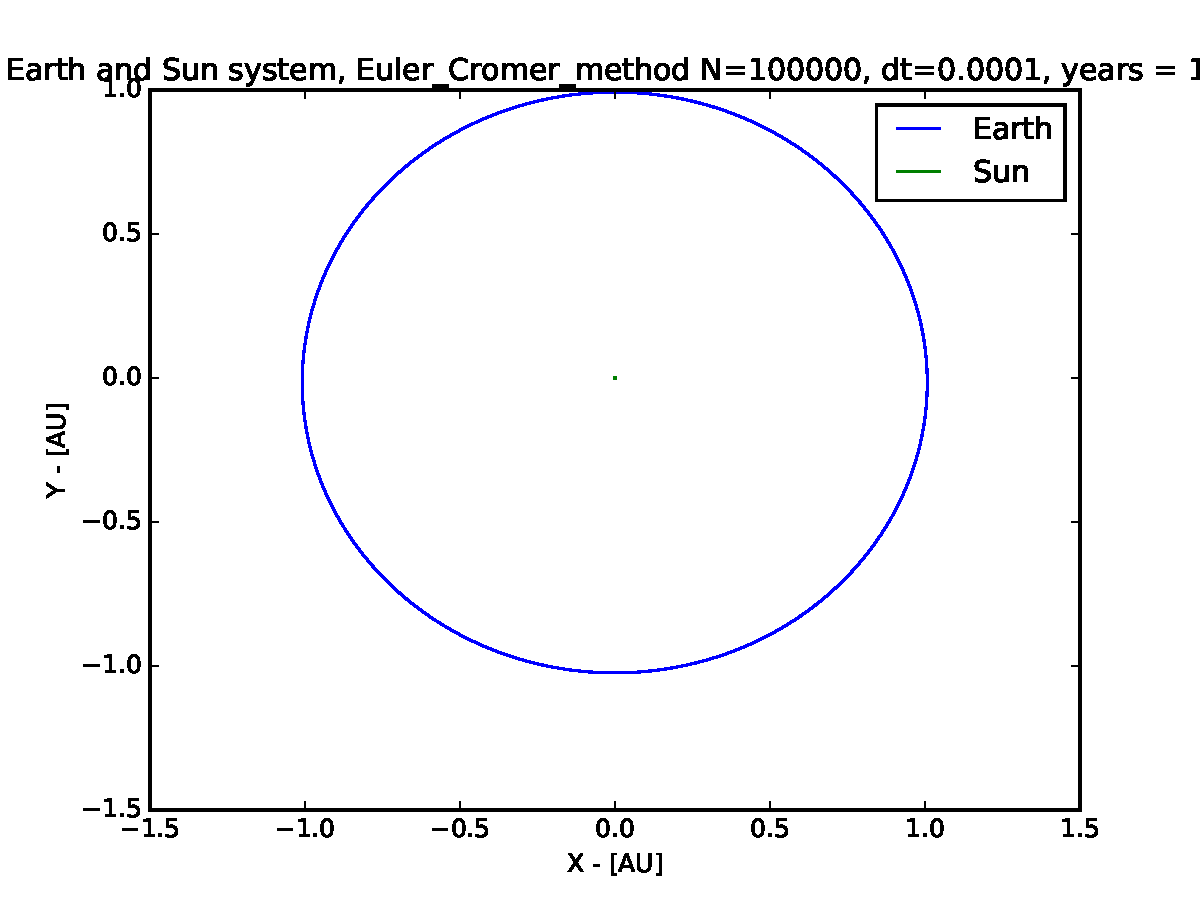
\includegraphics[width=\linewidth]{Plots/Earth_Sun_Euler_Cromer_method.pdf}
\caption{Earth-Sun system using Euler Cromer method}
\end{figure}

\end{document}